\chapter{Appendix }

\section{Neuron Parameters}

\begin{table}[h!]
\caption{Current-based LIF neuron parameters used for the converted CNN.}
\centering
\label{cnnlifparam}
\begin{tabularx}{0.65\textwidth}{|XX|}
\hline
Resting potential    		& -65 mV 		    \\
Membrane capacity    		& 1.0 nF 		     \\
Membrane time constant    	& 20.0 ms		             \\
Refractory period     		& 1.0 ms		                 \\
Offset current    			& 0.0 nA		              \\
Reset potential     		& -65.0 mV 	               \\
Spike threshold     		& -50.0 mV          \\\hline
\end{tabularx}
\end{table}

\begin{table}[h!]
\caption{Current-based LIF neuron parameters used for the converted DBN.}
\centering
\label{cubalifparam}
\begin{tabularx}{0.65\textwidth}{|XX|}
\hline
Resting potential    		& -65 mV 		    \\
Membrane capacity    		& 1.0 nF 		     \\
Membrane time constant    	& 1.0 ms		             \\
Refractory period     		& 10.0 ms		                 \\
Offset current    			& 1.0 nA		              \\
Reset potential     		& -53.0 mV 	               \\
Spike threshold     		& -52.0 mV          \\\hline
\end{tabularx}
\end{table}


\begin{table}[h!]
\caption{Conductance-based LIF neuron parameters used for the converted DBN.}
\centering
\label{cobalifparam}
\begin{tabularx}{0.65\textwidth}{|XX|}
\hline
Resting potential    			& -65 mV 		    \\
Membrane capacity    			& 1.0 nF 		     \\
Membrane time constant    		& 20.0 ms		             \\
Refractory period     			& 10.0 ms		                 \\
Offset current    				& 1.0 nA		              \\
Reset potential     			& -53.0 mV 	               \\
Spike threshold     			& -52.0 mV          \\
Inhibitory reversal potential  & 90.0 mV	              \\
Excitatory reversal potential  & -0.0 mV 	               \\\hline
\end{tabularx}
\end{table}
   
\pagebreak   
   
\section{Lateral Inhibition}   
   
 \begin{figure}[h!]
	\centering
	\begin{subfigure}[t]{.55\textwidth}
  		\centering
  		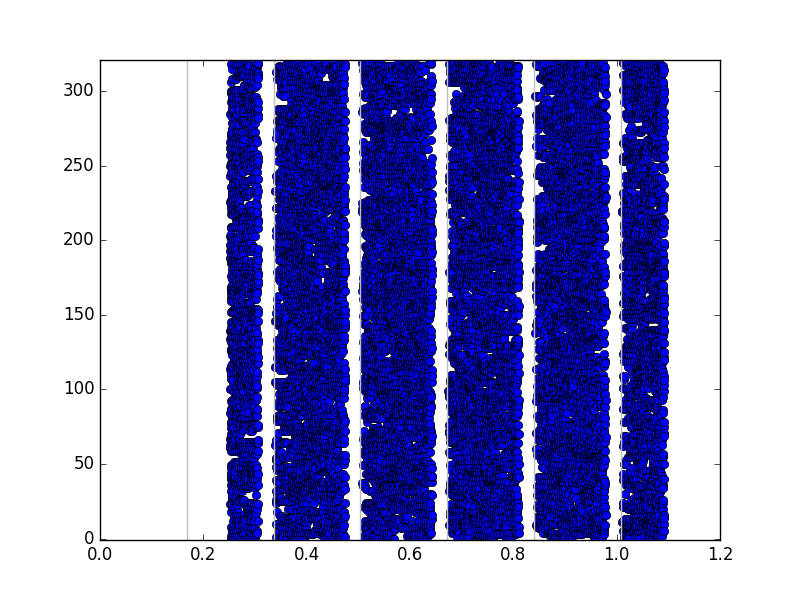
\includegraphics[width=.9\linewidth]{imgs/app/inhib_no.png}
  		\caption{Spikes without lateral inhibition.}
  		\label{fig:sub1}
	\end{subfigure}%
	
	\begin{subfigure}[t]{.55\textwidth}
  		\centering
  		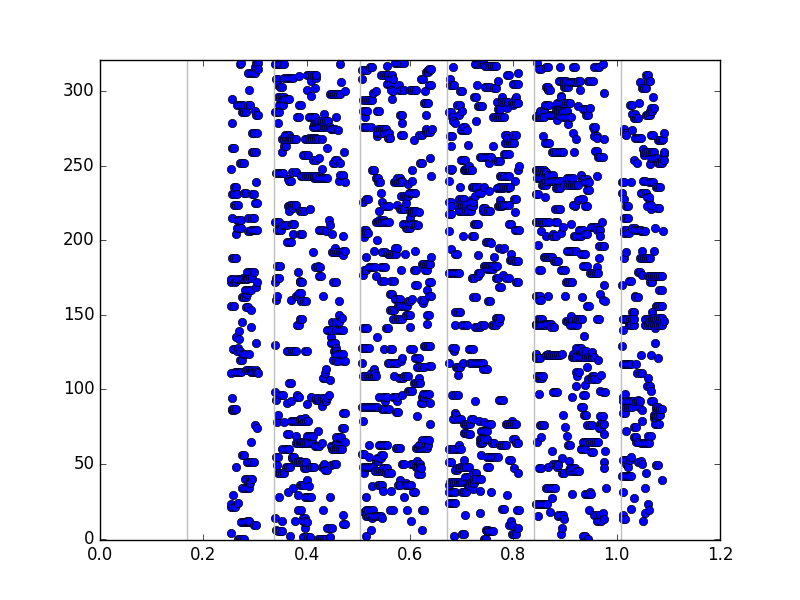
\includegraphics[width=.9\linewidth]{imgs/app/inhib_small.png}
  		\caption{Spikes with small lateral inhibition.}
  		\label{fig:sub2}
	\end{subfigure}
	
	\begin{subfigure}[t]{.55\textwidth}
  		\centering
  		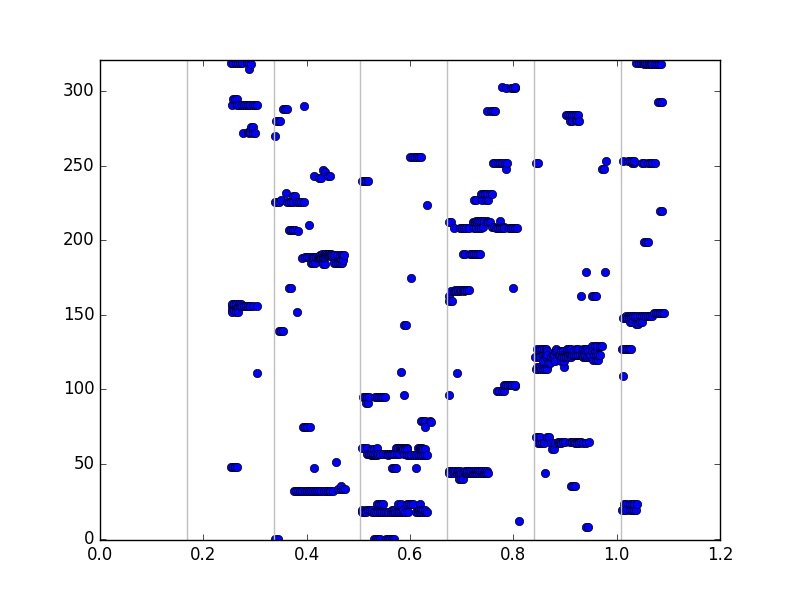
\includegraphics[width=.9\linewidth]{imgs/app/inhib_big.png}
  		\caption{Spikes with big lateral inhibition.}
  		\label{fig:sub2}
	\end{subfigure}
	\caption[Spikes in a hidden layer of a spiking RBM with different kinds of lateral inhibition.]{Spikes in a hidden layer of a spiking RBM with lateral inhibition. As the lateral inhibition increases, the activity becomes more sparse. In the case with big inhibitory weights, there are a few neurons dominating the activity allowing only a few different states of the network and thus poor mode switching in a training step. In a network with small inhibitory weights, there is sparse activity, but the network visits many different states in a simulation step and shows sufficient mode mixing. }
	\label{fig:dbnmixing}
\end{figure}
   
\section{Spiking DBN Architectures}   
   
 \begin{figure}[h!]
	\centering
	\begin{subfigure}[t]{.49\textwidth}
  		\centering
  		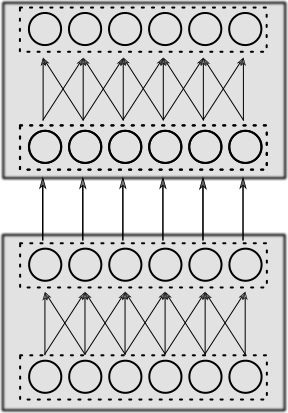
\includegraphics[width=.4\linewidth]{imgs/spike_dbn.png}
  		\label{fig:sub1}
  		\caption{DBN with distinct RBM layers.}
	\end{subfigure}%
	\begin{subfigure}[t]{.49\textwidth}
  		\centering
  		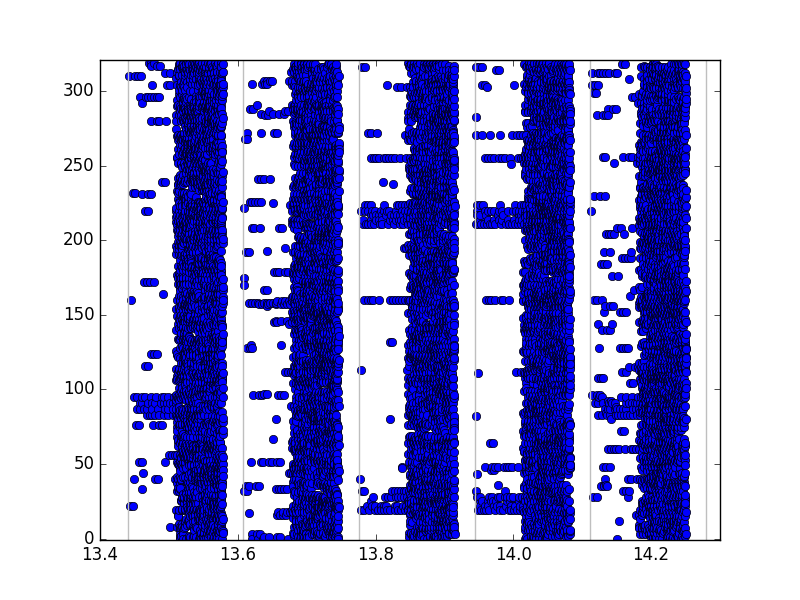
\includegraphics[width=.9\linewidth]{imgs/app/DBN_sp.png}
  		\label{fig:sub1}
	\end{subfigure}%
	
	
	\begin{subfigure}[t]{.49\textwidth}
  		\centering
  		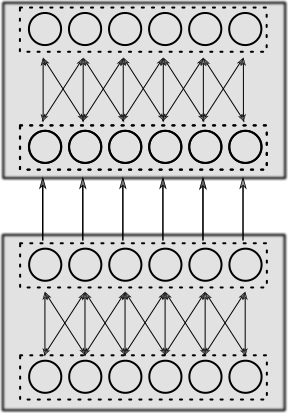
\includegraphics[width=.4\linewidth]{imgs/spike_dbm.png}
  		\label{fig:sub1}
  		\caption{DBN with distinct RBM layers, with bidirectional weights.}
	\end{subfigure}%
	\begin{subfigure}[t]{.49\textwidth}
  		\centering
  		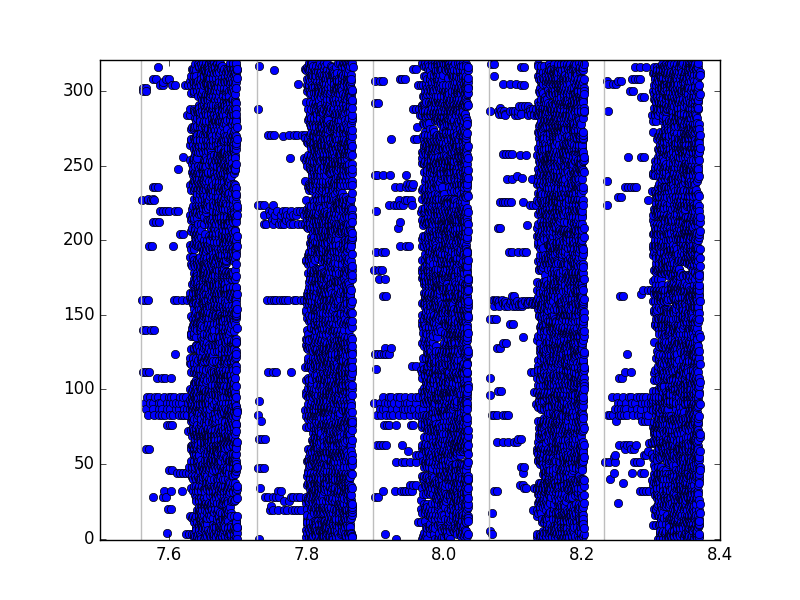
\includegraphics[width=.9\linewidth]{imgs/app/DBM_sp.png}
  		\label{fig:sub2}
	\end{subfigure}
	
	
	\begin{subfigure}[t]{.49\textwidth}
  		\centering
  		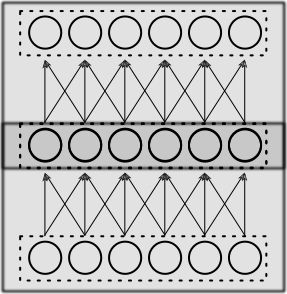
\includegraphics[width=.50\linewidth]{imgs/app/dbn_np_arch.png}
  		\label{fig:sub1}
  		 \caption{DBN with RBM directly stacked to each other.}
	\end{subfigure}%
	\begin{subfigure}[t]{.49\textwidth}
  		\centering
  		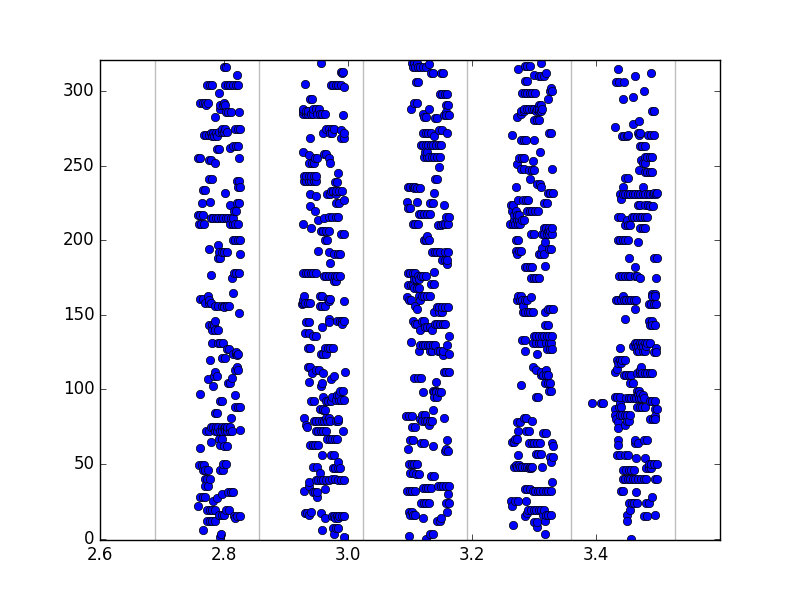
\includegraphics[width=.9\linewidth]{imgs/app/DBN_np_sp.png}
  		\label{fig:sub2}
	\end{subfigure}
	\caption[Activity in the visible layer of the top RBM in a DBNs with different architectures.]{Activity in the visible layer of the top RBM in a DBNs with different architectures. The first two architectures model separate RBM layers which are stacked by one-on-one forward connections from the hidden layer of the bottom RBM to the visible layer of the top RBM, while in the last architecture the RBMs are directly stacked, i.e. the hidden layer of the bottom RBM is the visible layer of the top RBM. While in the top two architectures, there are hardly any differences and the input is modelled correctly, due to top down influences the output of the bottom RBM gets distorted by activity in the hidden layer of the top RBM.}
	\label{fig:spikingdbnarch}
\end{figure}

\section{Synchronous Weight Updates} \label{fig:ecdnestconv}

For this thesis two different approaches were implemented. 

The first approach, as presented in Chapter \ref{c:ecdconv} and \ref{c:ecdexp}, synchronizes the weights at a discrete time step after a training sample is presented and processed.
This poses some similarities to the normal contrastive divergence algorithm since, due to discrete nature of artificial neural networks, the weights are updated and synchronized after the positive and negative phase.  

The second approach keeps the weights synchronized by applying the same STDP update to all synapses which share the same weight at the same time. 
Namely, if one synapses is updated by a local STDP rule, the update is shared with all tied synapses.
For the non-convolutional case i.e. only the weights of forward and backward synapses between the same neurons are shared, this leads to discriminative results, as shown in Figure \ref{fig:nestwwout}.

\begin{figure}[h!]

	\begin{subfigure}[t]{.49\textwidth}
		\centering
		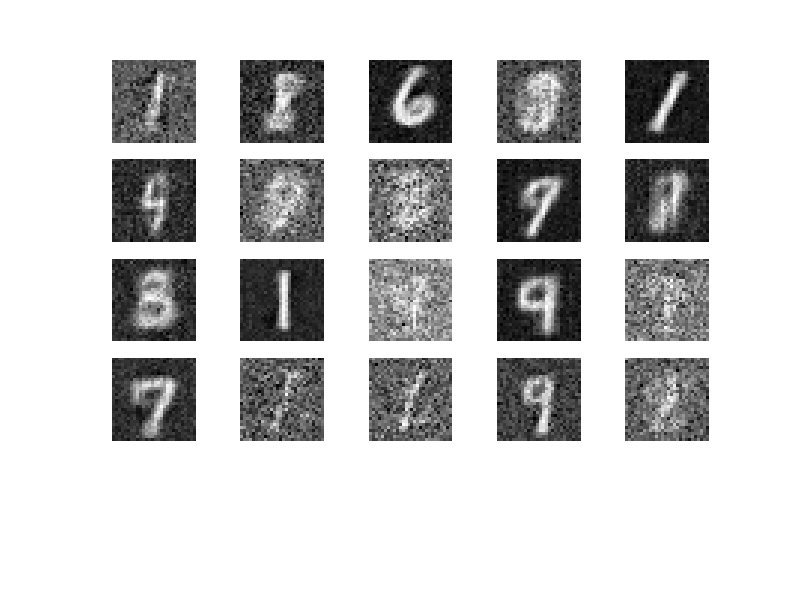
\includegraphics[width=.9\linewidth]{imgs/app/nest/ws.png}
		\caption{}
		\label{fig:sub12}
	\end{subfigure}
	\begin{subfigure}[t]{.49\textwidth}
  		\centering
  		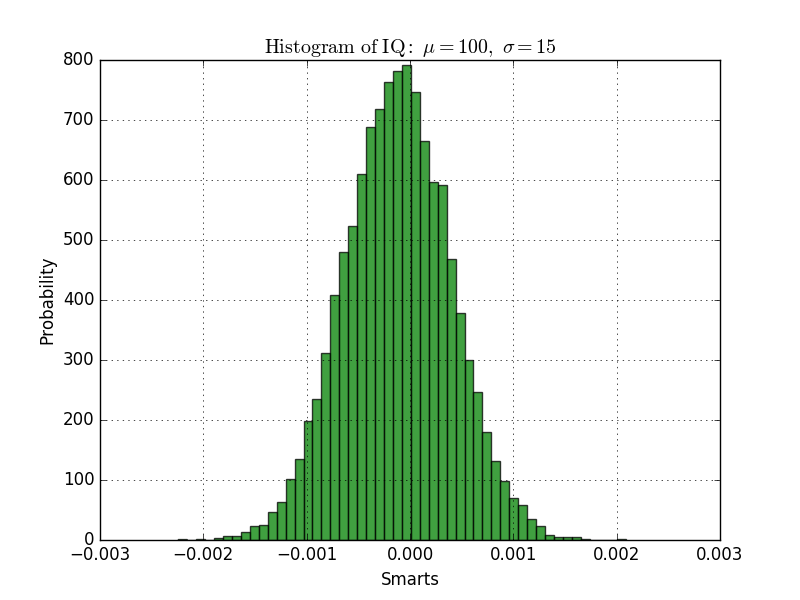
\includegraphics[width=.9\linewidth]{imgs/app/nest/w_hist_normal.png}
  		\caption{}
  		\label{fig:sub2}
	\end{subfigure}
	\caption[Weights with shared STDP weight updates and without any convolution.]{Weights with shared STDP weight updates and without any convolution. The weights are visualized in (a) as the filter matrices and in (b) as a histogram. }
	\label{fig:nestwwout}
\end{figure}	


In our case, the case with shared STDP updates with convolutions did not show any promising results. Although the learning rate was scaled accordingly, due to some self-facilitation and weight explosion, the weights become mostly negative as illustrated in Figure \ref{fig:ecdnestconv}.


 \begin{figure}[h!]
	\centering
	\begin{subfigure}[t]{.24\textwidth}
  		\centering
  		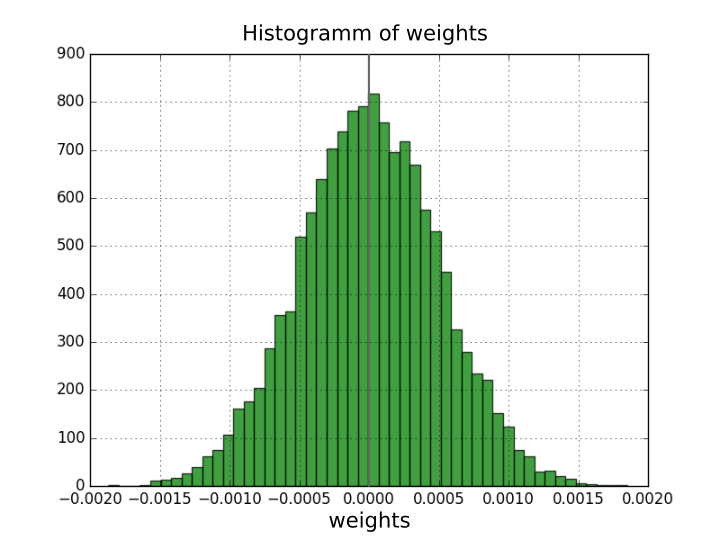
\includegraphics[width=.9\linewidth]{imgs/app/nest/w_hist_conv1.png}
  		\caption{}
  		\label{fig:sub1}
	\end{subfigure}%
	\begin{subfigure}[t]{.24\textwidth}
  		\centering
  		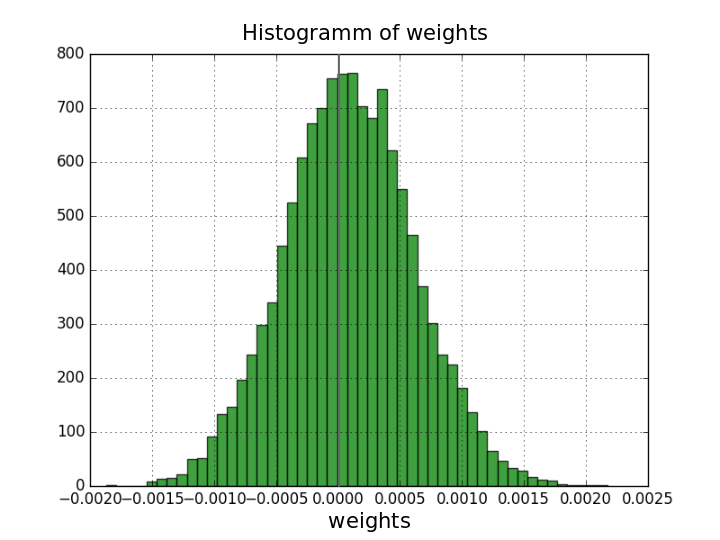
\includegraphics[width=.9\linewidth]{imgs/app/nest/w_hist_conv2.png}
  		\caption{}
  		\label{fig:sub2}
	\end{subfigure}
	\begin{subfigure}[t]{.24\textwidth}
  		\centering
  		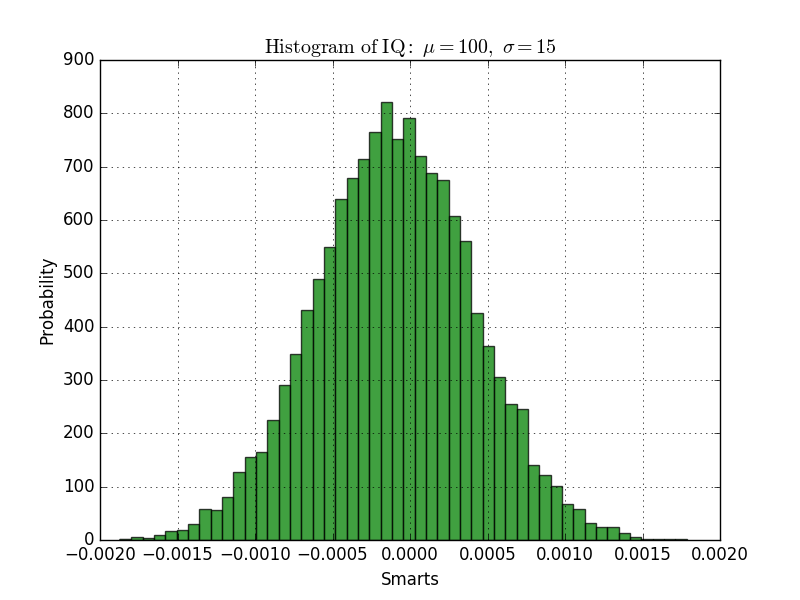
\includegraphics[width=.9\linewidth]{imgs/app/nest/w_hist_conv3.png}
  		\caption{}
  		\label{fig:sub2}
	\end{subfigure}
	\begin{subfigure}[t]{.24\textwidth}
  		\centering
  		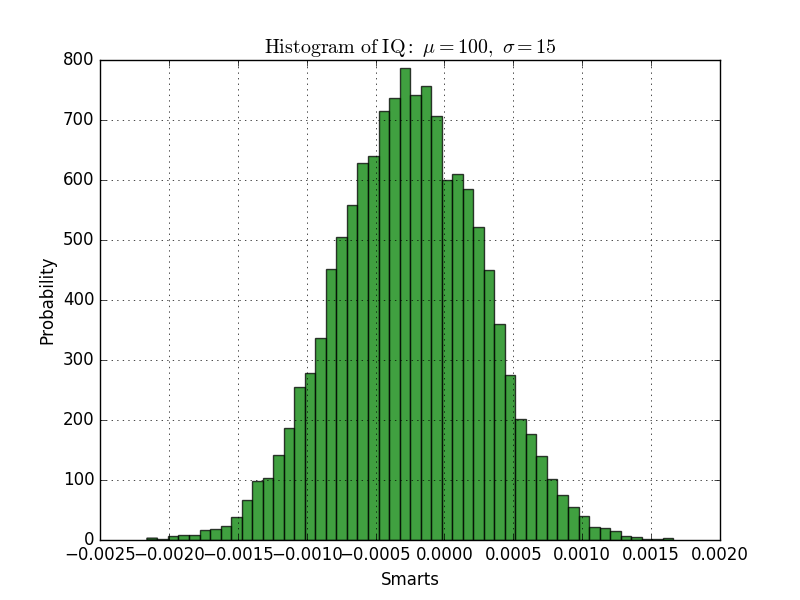
\includegraphics[width=.9\linewidth]{imgs/app/nest/w_hist_conv4.png}
  		\caption{}
  		\label{fig:sub2}
	\end{subfigure}
	\caption[Weights development for eCD with synchronous weight updates.]{Weights development for eCD with synchronous weight updates. The weight distribution in the beginning is shown in (a). After the positive phase (b) the weights increased a lot, which leads to a high decrement during the negative (c). During further training this trend continues until most weights are negative (d).}
	\label{fig:ecdnestconv}
\end{figure}

As a result, due to the mostly negative weights, this leads to a "dying-out" of the spike activity which is shown in Figure \ref{fig:ecdnestdieout} 

\begin{figure}[h!]
 	\centering
  	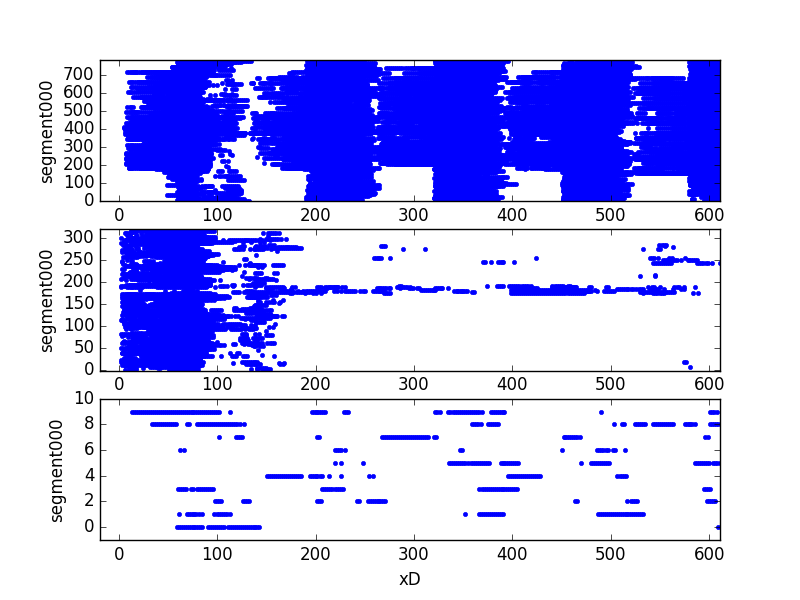
\includegraphics[width=.4\linewidth]{imgs/app/nest/spikes_conv.png}
  	\caption[Spikes activity during convolutional eCD with synchronous weight updates.]{Spikes activity during convolutional eCD with synchronous weight updates. After a few training samples are presented the spiking activity decreases, due to the decrement of the synaptic weights.}
  	\label{fig:ecdnestdieout}
\end{figure}

Thus, no learning happens and the weights become not very discriminative (compare Figure \ref{fig:ecdnestwnot}).


\begin{figure}[h!]
 	\centering
  	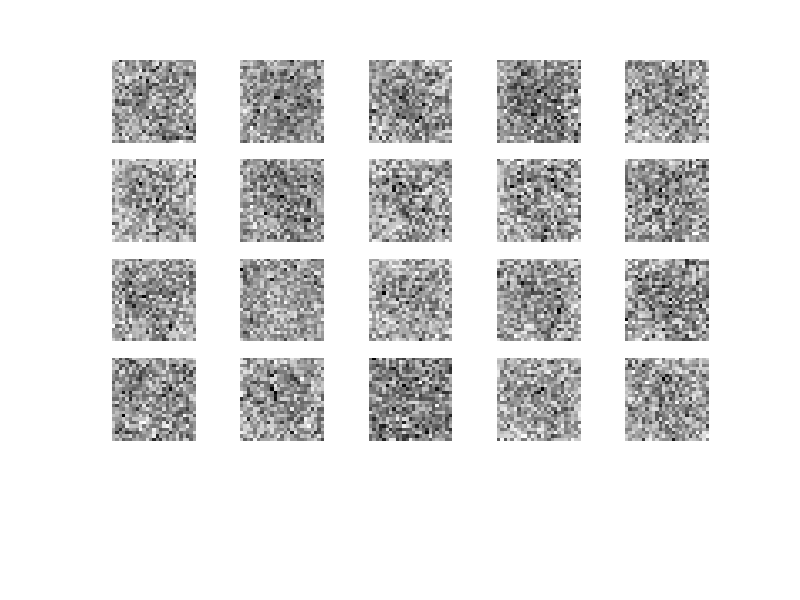
\includegraphics[width=.4\linewidth]{imgs/app/nest/w_not.png}
  	\caption{Learned weights for convolutional eCD with synchronous weight updates.}
  	\label{fig:ecdnestwnot}
\end{figure}

Increasing the learning rate to increase the weights leads to a few strong positive weights, while the majority of the weights still become negative leading to no good results either (Fig. \ref{fig:ecdnestwnot}).


\begin{figure}[h!]
 	\centering
  	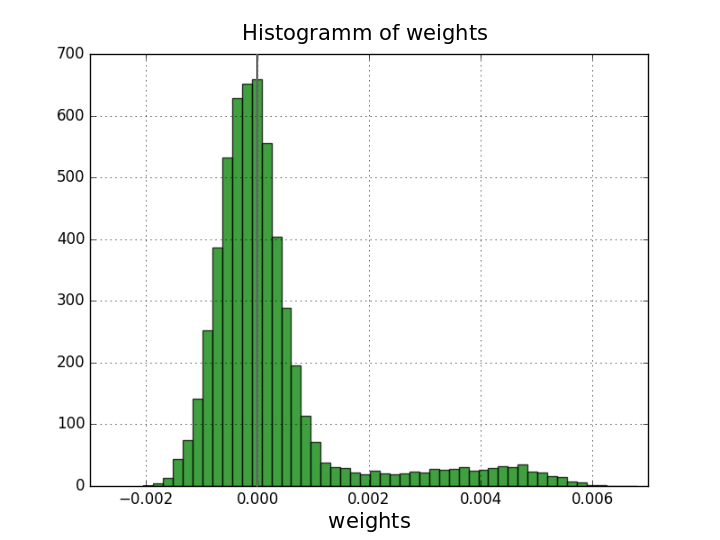
\includegraphics[width=.4\linewidth]{imgs/app/nest/w_hist_conv_lr.png}
  	\caption[Weight histogram for convolutional eCD with synchronous weight updates and an increased learning rate during the positive phase.]{Weight histogram for convolutional eCD with synchronous weight updates and an increased learning rate during the positive phase. This leads to a division of the weights into a few very positive weights and many negative weights. }
  	\label{fig:ecdnestwnot}
\end{figure}

Further research on this topic could indicate whether a fine-tuned learning rate or a dynamic learning rate decay or adaptation could be a sound remedy to this problem. 

%
% \begin{figure}[h!]
%	\centering
%	\begin{subfigure}[t]{.24\textwidth}
%  		\centering
%  		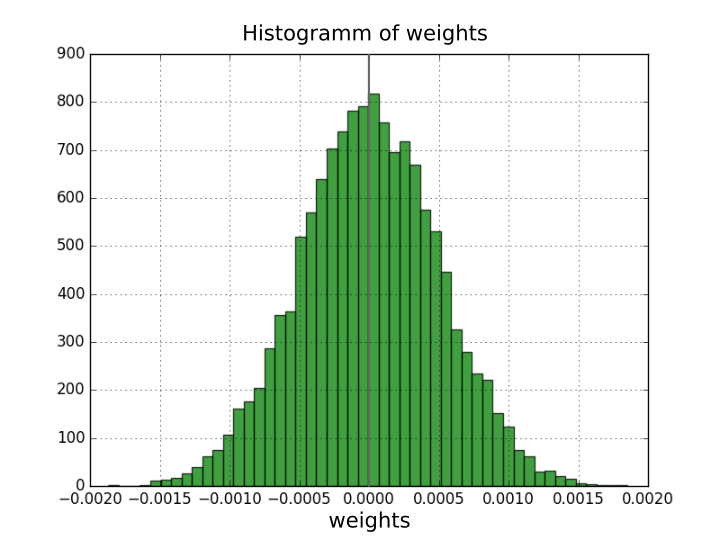
\includegraphics[width=.9\linewidth]{imgs/app/nest/w_hist_conv1.png}
%  		\caption{Weights at the beginning.}
%  		\label{fig:sub1}
%	\end{subfigure}%
%	\begin{subfigure}[t]{.24\textwidth}
%  		\centering
%  		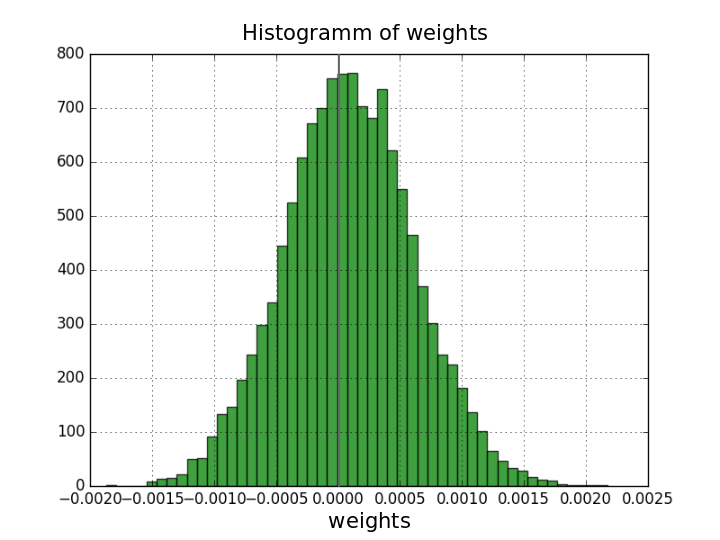
\includegraphics[width=.9\linewidth]{imgs/app/nest/w_hist_conv2.png}
%  		\caption{Weights after first positive phase.}
%  		\label{fig:sub2}
%	\end{subfigure}
%	\begin{subfigure}[t]{.24\textwidth}
%  		\centering
%  		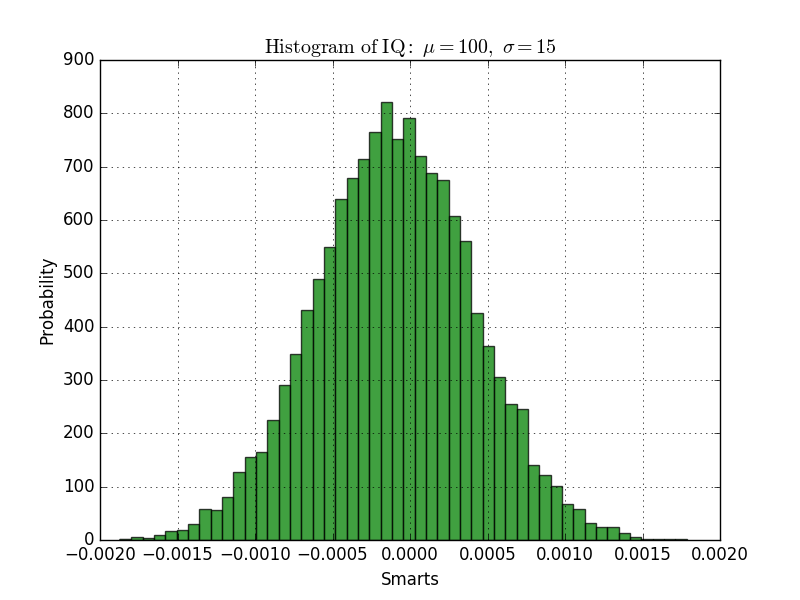
\includegraphics[width=.9\linewidth]{imgs/app/nest/w_hist_conv3.png}
%  		\caption{Weights after first negative phase.}
%  		\label{fig:sub2}
%	\end{subfigure}
%	\begin{subfigure}[t]{.24\textwidth}
%  		\centering
%  		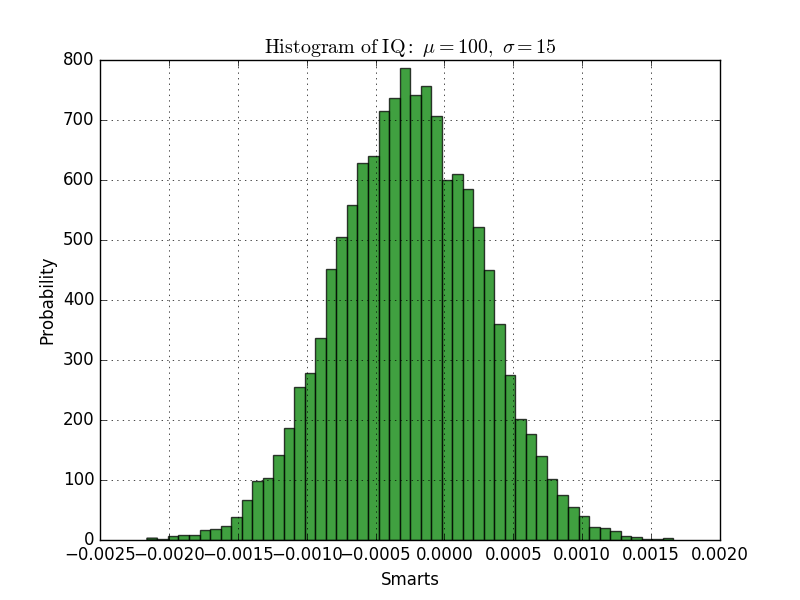
\includegraphics[width=.9\linewidth]{imgs/app/nest/w_hist_conv4.png}
%  		\caption{Weights after a few training steps.}
%  		\label{fig:sub2}
%	\end{subfigure}
%	
%
%	\begin{subfigure}[t]{.24\textwidth}
%  		\centering
%  		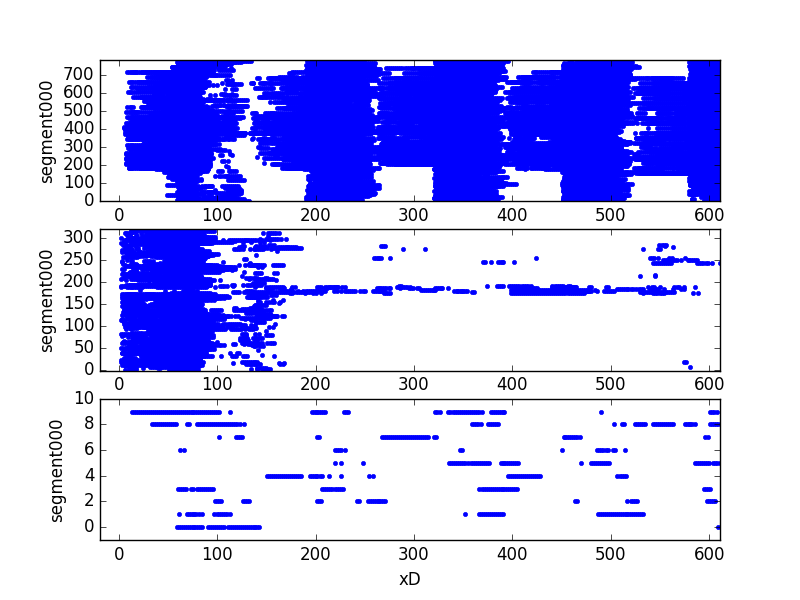
\includegraphics[width=.9\linewidth]{imgs/app/nest/spikes_conv.png}
%  		\caption{Spikes activity development.}
%  		\label{fig:sub2}
%	\end{subfigure}
%	
%	
%	\begin{subfigure}[t]{.24\textwidth}
%  		\centering
%  		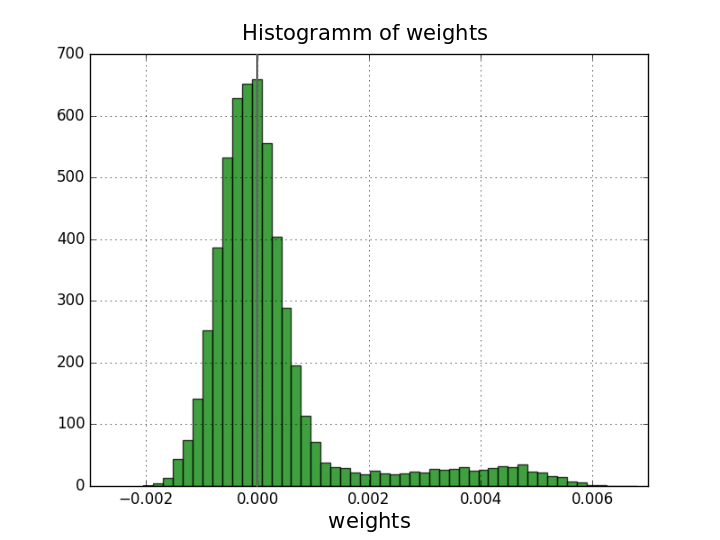
\includegraphics[width=.9\linewidth]{imgs/app/nest/w_hist_conv_lr.png}
%  		\caption{Weights after training with different positive and negative learning rates.}
%  		\label{fig:sub2}
%	\end{subfigure}
%	
%	\begin{subfigure}[t]{.24\textwidth}
%  		\centering
%  		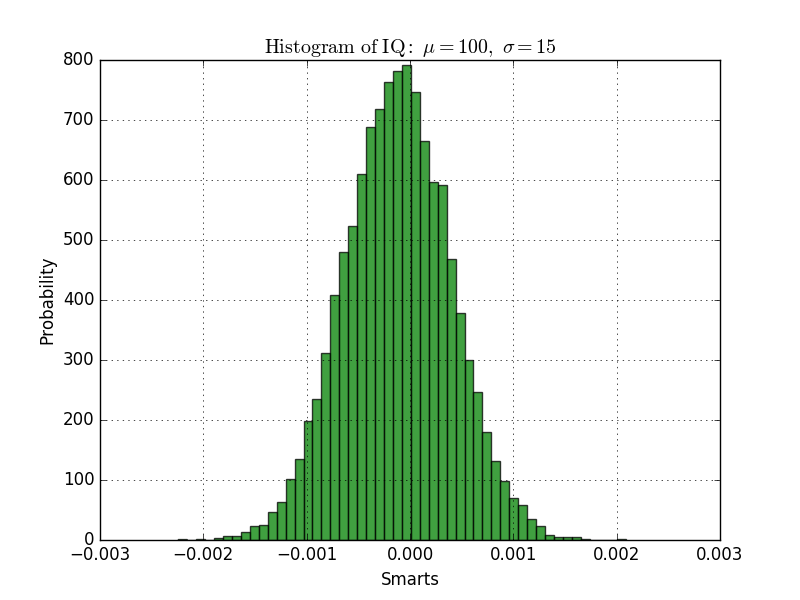
\includegraphics[width=.9\linewidth]{imgs/app/nest/w_hist_normal.png}
%  		\caption{Weights without any synchronization.}
%  		\label{fig:sub2}
%	\end{subfigure}	
%	
%	\caption{Weights development for eCD with synchronous weight updates. The first column shows the development. After the positive the weights increased a lot, which leads to a high decrement during the negative which leads to a "dying out" of the spikes, which is visualized in the second column. Using an increased positive phase with a higher learning rate, does not solve the problem and leads to a division of the weights into a few very positive weights and many negative weights. In contrast to this a "normal" weight distribution without any weight synchronization in presented in the last column. }
%	\label{fig:ecdnestconv}
%\end{figure}

